\documentclass{article}

% if you need to pass options to natbib, use, e.g.:
%     \PassOptionsToPackage{numbers, compress}{natbib}
% before loading neurips_2019

% ready for submission
% \usepackage{neurips_2019}

% to compile a preprint version, e.g., for submission to arXiv, add add the
% [preprint] option:
%     \usepackage[preprint]{neurips_2019}

% to compile a camera-ready version, add the [final] option, e.g.:
\usepackage[final]{neurips_2019}

% to avoid loading the natbib package, add option nonatbib:
%     \usepackage[nonatbib]{neurips_2019}

\usepackage[utf8]{inputenc} % allow utf-8 input
\usepackage[T1]{fontenc}    % use 8-bit T1 fonts
\usepackage{hyperref}       % hyperlinks
\usepackage{url}            % simple URL typesetting
\usepackage{booktabs}       % professional-quality tables
\usepackage{amsmath}
\usepackage{amsfonts}       % blackboard math symbols
\usepackage{nicefrac}       % compact symbols for 1/2, etc.
\usepackage{microtype}      % microtypography
\usepackage{graphicx}
\usepackage{wrapfig}
\usepackage{bm}
%\allowdisplaybreaks
\usepackage{lipsum}
\newcommand{\indep}{\rotatebox[origin=c]{90}{$\models$}}

\title{1RT705: Group 5682}

% The \author macro works with any number of authors. There are two commands
% used to separate the names and addresses of multiple authors: \And and \AND.
%
% Using \And between authors leaves it to LaTeX to determine where to break the
% lines. Using \AND forces a line break at that point. So, if LaTeX puts 3 of 4
% authors names on the first line, and the last on the second line, try using
% \AND instead of \And before the third author name.

%\author{%
%	David S.~Hippocampus\thanks{Use footnote for providing further information
%		about author (webpage, alternative address)---\emph{not} for acknowledging
%		funding agencies.} \\
%	Department of Computer Science\\
%	Cranberry-Lemon University\\
%	Pittsburgh, PA 15213 \\
%	\texttt{hippo@cs.cranberry-lemon.edu} \\
	% examples of more authors
	% \And
	% Coauthor \\
	% Affiliation \\
	% Address \\
	% \texttt{email} \\
	% \AND
	% Coauthor \\
	% Affiliation \\
	% Address \\
	% \texttt{email} \\
	% \And
	% Coauthor \\
	% Affiliation \\
	% Address \\
	% \texttt{email} \\
	% \And
	% Coauthor \\
	% Affiliation \\
	% Address \\
	% \texttt{email} \\
%}

\begin{document}
	
	\maketitle
%	
%	\begin{abstract}
%		The abstract paragraph should be indented \nicefrac{1}{2}~inch (3~picas) on
%		both the left- and right-hand margins. Use 10~point type, with a vertical
%		spacing (leading) of 11~points.  The word \textbf{Abstract} must be centered,
%		bold, and in point size 12. Two line spaces precede the abstract. The abstract
%		must be limited to one paragraph.
%	\end{abstract}
	
	\section{Outline}
	The layout of this report is designed to answer the questions Q1 through Q10 in ascending order. The title of each section is named so it describes what questions it will give answers to.
	\section{Modeling (Q1-Q3)}
	\label{sec:modeling}
	The \textit{TrueSkill} Bayesian model for one match can be formulated as
	
	\begin{subequations}
	\begin{align}
	p(s_1) &= \mathcal{N}(s_1; \mu_1, \sigma_1^2),\\
	p(s_2) &= \mathcal{N}(s_2; \mu_2, \sigma_2^2),\\
	p(t|s_1, s_2) &= \mathcal{N}(t; s_1-s_2, \sigma_t^2),\\
	y &= \text{sign}(t),
	\end{align}\label{eqn:model}
	\end{subequations}
	where $ \{\mu_1,\mu_2,\sigma_1,\sigma_2,\sigma_t\} $ are the hyperparameters to set. Microsoft states\footnote{\url{https://www.microsoft.com/en-us/research/project/trueskill-ranking-system/} (accessed: 2019-10-03)} that in their implementation of the \textit{TrueSkill} model, the default value for new players is $ \mu=25, \sigma=8.3333 $ and that the \textit{TrueSkill} value for that player is $25-3\cdot8.3333=0$, being the conservative estimate of the player's skill. 
	
	Gathering $ s_1 $ and $ s_2 $ as $s = (s_1, s_2)$, the conditional distribution of the skills $p(s_1, s_2|t,y)$ can be computed using Corollary 1 from the lectures of the course:
	
	\begin{subequations}
	\begin{align}
		p(s | t, y) &= p(s | t) = \mathcal{N}\Big( s;~\mu_{s|t},\,\Sigma_{s|t} \Big),\\
		\mu_{s|t} &= \Sigma_{s|t}\Big(\Sigma_s^{-1} \mu_s + M^T\Sigma_{t|s}^{-1}t\Big),\\
		\Sigma_{s|t} &= \Big( \Sigma_s^{-1} + M^T\Sigma_{t|s}^{-1}M \Big)^{-1},
	\end{align}
	\end{subequations}
	where the covariance matrix for $t$ given $s$ is just $\Sigma_{t|s}=\sigma_t^2$ from the model \eqref{eqn:model}, the matrix $M$ is $[1, -1]$ so that $M^Ts = s_1 - s_2$, the covariance matrix for s is $\Sigma_s = \begin{bmatrix}
	\sigma_1^2 & 0\\ 0 & \sigma_2 \end{bmatrix}$ and the mean vector for s is $\mu_s = [\mu_1, \mu_2]^T$.
	
	The full conditional distribution for the outcome $t$ becomes a truncated normal distribution, due to the information from $y$ that indicates the sign of the variable $t$:
	\begin{align}
	p(t|s_1, s_2, y) = \mathcal{TN}(t;~s_1-s_2, \sigma_t^2, y),
	\end{align}
	where we let the notation $\mathcal{TN}(x;~\mu, \sigma^2, a)$ be the normal distribution $\mathcal{N}(x;~\mu, \sigma^2)$ while the pdf is zero for $ x<0 $ if $ y=1 $, or zero for $ x>0 $ if $ y=-1 $.
	
	\begin{wrapfigure}[6]{r}{0.3\textwidth}
		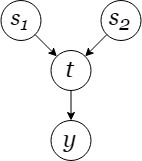
\includegraphics[width=\linewidth]{bayes4}
		\caption{A Bayesian network of the model in \eqref{eqn:model}.}
		\label{fig:bayes_n}
	\end{wrapfigure}
	
	The marginal probability of $ y=1 $ is computed by marginalizing the joint distribution that can be formulated from the Bayesian network in figure \ref{fig:bayes_n}.
	
	\begin{align}
	\begin{split}
	p(y=1) 	&= \int_{s_1}\int_{s_2}\int_t p(s_1, s_2, t, y=1)\,ds_1\,ds_2\,dt=\\
			&= \int_{s_1}p(s_1)\int_{s_2}p(s_2)\int_t p(t|s_1,s_2)p(y=1|t)\,dt\,ds_2\,ds_1\\
			&= \int_{s_1}p(s_1)\int_{s_2}p(s_2)\int_0^\infty p(t|s_1,s_2)\,dt\,ds_2\,ds_1\\
			&= \int_{s_1}p(s_1)\int_{s_2}p(s_2) (1 - D(t=0|s_1,s_2))\,ds_2\,ds_1\\
			&= (1-D(t=0|s_1,s_2))\int_{s_1}p(s_1)ds_1\int_{s_2}p(s_2)ds_2\\
			&= (1-D(t=0|s_1,s_2)) = (1 - \dfrac{1}{2}(1+\text{erf}\Big(\dfrac{0-(s_1-s_2)}{\sigma_t\sqrt{2}}\Big)))\\
			&= \dfrac{1}{2}\Big(1 - \text{erf}\Big(\dfrac{s_2-s_1}{\sigma_t\sqrt{2}}\Big)\Big),
	\end{split}
	\end{align}
	where $ D(t|s_1,s_2) = \frac{1}{2}(1+\text{erf}(\frac{t-(s_1-s_2)}{\sigma_t\sqrt{2}}))$ is the cumulative distribution function of $p(t|s_1,s_2)$ [4].
	
	A Bayesian network of the model \eqref{eqn:model} is presented in figure \ref{fig:bayes_n}, from which we together with rules of independence in Bayesian networks [1] can observe two conditionally independent sets of variables as:
	\begin{align}
		s_1 \,\indep \, s_2 ~|~ \emptyset, \\
		s_1 \,\indep \, y ~|~ t.
	\end{align}
	
	\section{Gibbs Sampling (Q4)}
	\begin{wrapfigure}[17]{r}[11pt]{0.5\textwidth}
		\begin{center}
			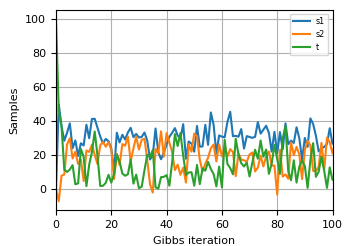
\includegraphics[width=\linewidth]{q_4_samples}
		\end{center}
		\caption{\footnotesize{Samples of the variables $ s_1,s_2,t $ for 100 Gibbs sampler iterations.}}
		\label{fig:q_4_1}
	\end{wrapfigure}
	
	A Gibbs sampler was implemented to estimate the posteriors of the skills given the outcome $y$ of one match. The results discussed in this sections were generated using the default \textit{TrueSkill} values for $ \mu_1=\mu_2=25, \sigma_1=\sigma_2=25/3 $ and with $ \sigma_t^2=25/3 $.
	
	The initialization of the Gibbs sampler consists of choosing a value for $t_0$. Figure \ref{fig:q_4_1}illustrates the propagation of the samples over the first 100 iterations of the Gibbs sampler for $t_0=100$ (i.e., player 1 wins by a huge margin -- in terms of football) and the other parameters set as discussed in section \ref{sec:modeling} and assuming $y=1$. From this plot, a burn-in of 50 samples seems reasonable, and it showed consistency over independent simulations.	
	
	The posterior distributions in figure \ref{fig:gibbs_mp_compare} illustrates how the mean increased and decreased for the winning and losing players, respectively.
	The standard deviation decreased for both players.

	The histograms in figure \ref{fig:q_4_2} illustrates that the choice of $K=450$ samples after the burn-in period of $50$ samples is very similar to $K=950$, while running in less than half that simulation's time. For the following experiments, $K=450$ is used together with the $50$ samples burn-in period. For the considered problems, there is only a couple of hundred measurements to consider, so the total simulation time is in the matter of minutes with this number of Gibbs sampler iterations. 
	
	\begin{wrapfigure}[24]{r}{0.5\textwidth}
		\begin{center}
		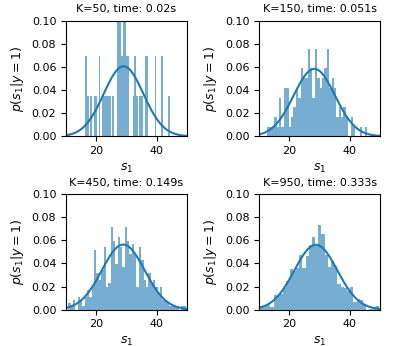
\includegraphics[width=\linewidth]{q_4_2_final}
		\end{center}
		\caption{Histograms of the samples (post burn-in) and the estimated posteriors for different values of $K$. The mean and standard deviation of the posteriors were estimated as the empirical mean and standard deviation of the samples from the Gibbs sampler.}
		\label{fig:q_4_2}
	\end{wrapfigure}
		
	\section{Assumed Density Filtering and Predictions (Q5-Q6)}
	The Gibbs sampler implementation was used to sequentially process match results from the \texttt{SerieA} dataset.
	Before simulation, all teams started out with the same skill distributions, with mean and standard deviation set to $ \mu=25, \sigma=25/3 $.
	
	Sequentially processing the matches from the \texttt{SerieA} dataset gave the final rankings as presented in table \ref{tab:q4}, together with the results generated using message passing.
	Alongside each skill's mean $\mu$ and standard deviation $ \sigma $ is the conservative estimate $\mu - 3\sigma$, by which the table is sorted in descending order.
	Note how Inter had lower expected skill than Milan, but the lower standard deviation cause the conservative estimate to rank them higher.
	
	By processing the matches in reverse order, the final rankings are different from before because the model used takes into account what skill distribution the teams have before the match, and playing matches in different order causes the priors to change between the Gibbs sampler simulations. The final rankings for this processing can be found in table \ref{tab:q4_rev} in the appendix.
	
	Before each match was simulated, the outcome was predicted. The correct prediction rate (disregarding draws) was computed in two ways: using the expected skills, and using the conservative estimates. The methods gave 62.5\% and 63.2\% correct predictions, respectively. This experiments demonstrates that doing this sequential Gibbs sampling processing can be better than guessing. 
	The implementation does not allow draw as a prediction, and therefore including drawn matches in the predictions as incorrect predictions reduces the correct prediction rates to 44.7\% and 45.2\%.

	\section{Factor Graphs and Message-Passing (Q7-Q8)}
	\begin{wrapfigure}[10]{l}{0.25\linewidth} % factor graph
		\centering
		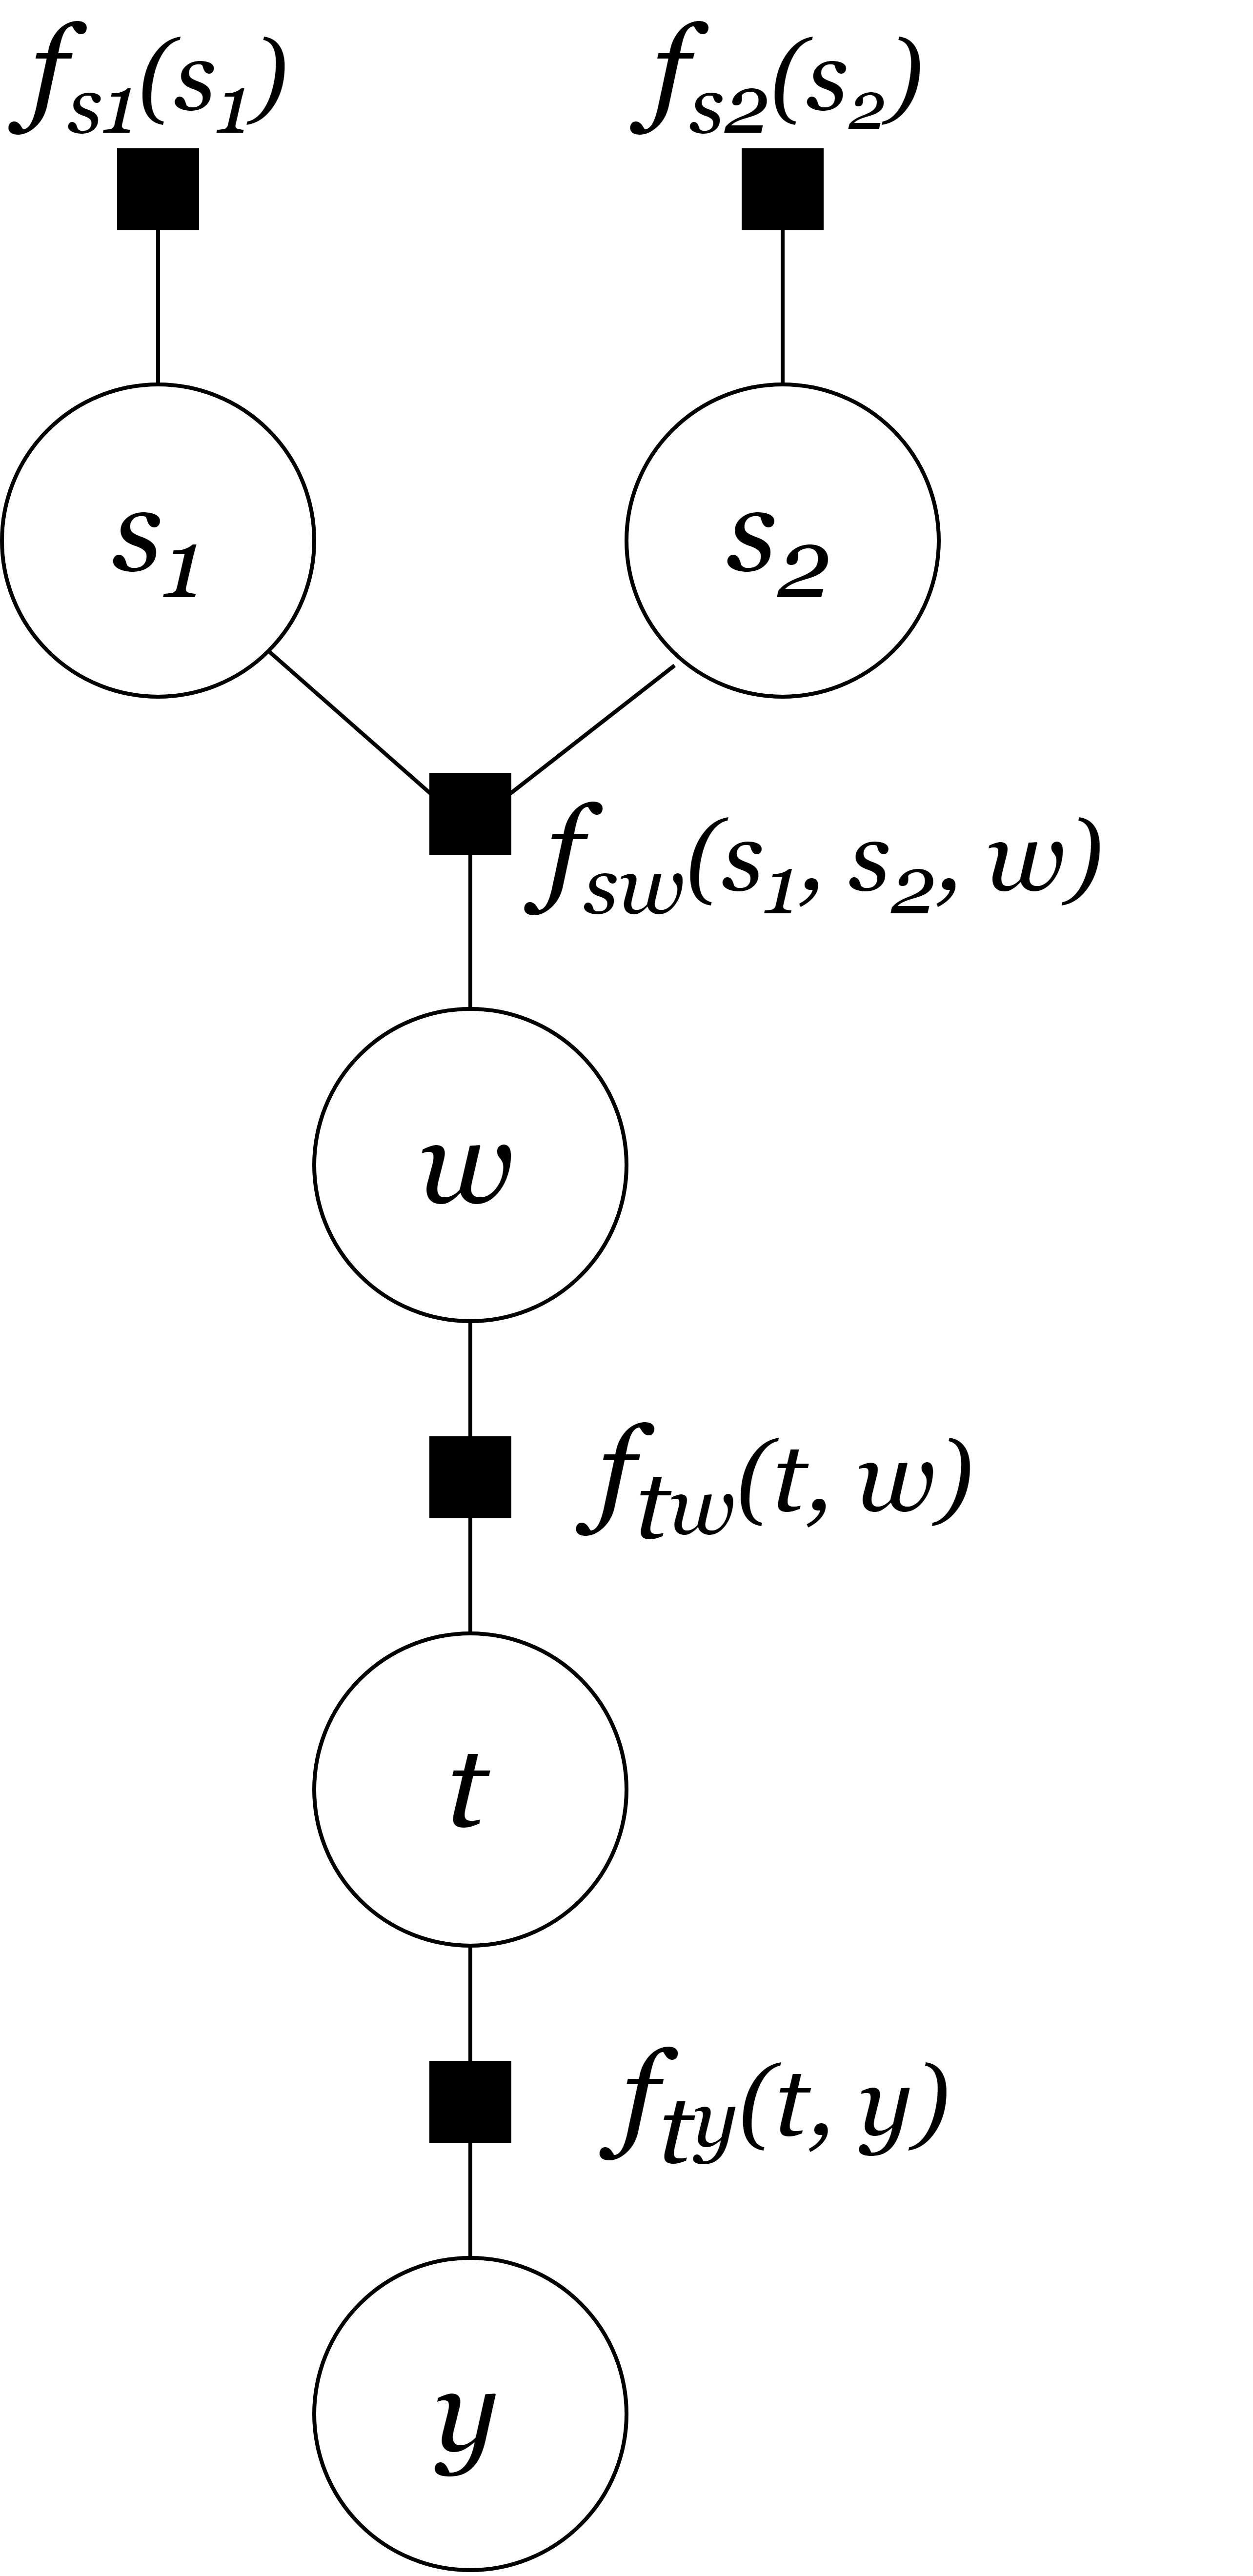
\includegraphics[width=\linewidth]{factor_graph}
		\caption{Factor graph of the model in \eqref{eqn:model}.}
		\label{fig:factor_graph}
	\end{wrapfigure}
	
	A factor graph was created for the model in \eqref{eqn:model}, and is illustrated in figure \ref{fig:factor_graph}, where the factor node functions are defined as:
		\begin{subequations}
		\begin{align}
			f_{s1}(s_1) &= \mathcal{N}(s_1; \mu_1, \sigma_1^2),\\
			f_{s2}(s_2) &= \mathcal{N}(s_2; \mu_2, \sigma_2^2),\\
			f_{sw}(s_1, s_2, w) &= \delta(w-(s_1-s_2)),\\
			f_{tw}(t,w) &= \mathcal{N}(t; w, \sigma_t^2),\\
			f_{ty}(t,y) &= \delta(\text{sign}(t)-y).
		\end{align}
		\end{subequations}
	When an observation is made in node $y$, a message passing protocol computes the posterior distributions $ p(s_1|y), p(s_2|y) $ as described in appendix \ref{app:message_passing}. From that protocol, the posteriors become:
	\clearpage
	\begin{subequations}\label{eqn:posterior_MP}
	\begin{align}
	p(s_1|y) &= \mathcal{N}(s_1; \dfrac{\mu_1(\hat{\sigma}_w^2 + \sigma_2^2) + (\mu_2 + \hat{\mu}_{tw})\sigma_1^2}{\sigma_1^2+\hat{\sigma}_w^2 + \sigma_2^2}, \dfrac{\sigma_1^2 ( \hat{\sigma}_w^2 +  \sigma_2^2)}{\sigma_1^2+\hat{\sigma}_w^2 + \sigma_2^2}),\\
	%
	p(s_2|y) &= \mathcal{N}(s_2; \dfrac{\mu_2(\hat{\sigma}_w^2 + \sigma_1^2) + (\mu_1 - \hat{\mu}_{tw})\sigma_2^2}{\sigma_1^2+\hat{\sigma}_w^2 + \sigma_2^2}, \dfrac{\sigma_2^2( \hat{\sigma}_w^2  + \sigma_1^2)}{\sigma_1^2+\hat{\sigma}_w^2 + \sigma_2^2}),
	\end{align}
	\end{subequations}
	where the moments $ \hat{\mu}_{tw} $ and $ \hat{\sigma}_{w}^2 $ comes from moment matching followed by division by normal distributions in the node $ t $.

		\begin{wrapfigure}[19]{l}{0.5\textwidth} % posteriors comparison
			\centering
			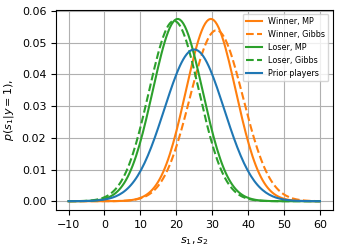
\includegraphics[width=\linewidth]{q_8_1st}
			\caption{\footnotesize{Posterior distributions of $ s_1 $ and $ s_2 $ after simulating one match where player 1 wins ($ y=1 $). The posteriors from Gibbs sampling and message passing (MP) are different from each other.} }
			\label{fig:gibbs_mp_compare}
		\end{wrapfigure}
	The message passing protocol was implemented in Python and posteriors were generated after simulating one win.
	The posteriors generated are shown together with the Gibbs samplers posterior distributions in figure \ref{fig:gibbs_mp_compare}.
	The graphs in the figure illustrates how if the prior variances are equal, their posterior variances will also be equal. 
	This is consistent with equation \eqref{eqn:posterior_MP}.
	
		\begin{table}[t]
			\caption{Mean, variance and conservative estimate of each team's skill after all match data was used. Final rankings are generated using Gibbs sampling and message passing, respectively. Initial values for all teams were set to $ \mu=25, \sigma=25/3 $ and the result variance was also set to $ \sigma_t=25/3 $. }
			\label{tab:q4}
			\centering
			\footnotesize
			\begin{tabular}{lrrr|lrrr}
				\toprule
				\multicolumn{4}{c}{Gibbs sampling} & \multicolumn{4}{c}{Message passing} \\
				\midrule
				Team     		& $ \mu $ & $ \sigma $ & $ \mu - 3\sigma $ & Team & $ \mu $ & $ \sigma $ & $ \mu-3\sigma $\\
				\midrule
				Juventus   &  34.95  &  2.94  &  26.14  &  Juventus    &  34.10  &  2.75  & 25.86 \\
				Napoli     &  31.97  &  2.56  &  24.30  &  Napoli      &  31.93  &  2.47  & 24.52 \\
				Inter      &  29.93  &  2.06  &  23.76  &  Milan       &  30.81  &  2.52  & 23.24 \\
				Milan      &  30.44  &  2.34  &  23.41  &  Atalanta    &  29.77  &  2.25  & 23.03 \\
				Atalanta   &  28.39  &  1.87  &  22.79  &  Inter       &  29.57  &  2.31  & 22.64 \\
				Torino     &  29.09  &  2.40  &  21.88  &  Roma        &  28.88  &  2.38  & 21.75 \\
				Roma       &  27.91  &  2.28  &  21.05  &  Torino      &  29.33  &  2.56  & 21.66 \\
				Lazio      &  26.89  &  2.04  &  20.77  &  Lazio       &  26.47  &  2.21  & 19.84 \\
				Sampdoria  &  24.69  &  2.22  &  18.03  &  Sampdoria   &  24.76  &  2.17  & 18.25 \\
				Spal       &  22.91  &  1.83  &  17.40  &  Spal        &  23.32  &  2.29  & 16.44 \\
				Bologna    &  24.22  &  2.53  &  16.63  &  Bologna     &  23.50  &  2.35  & 16.44 \\
				Sassuolo   &  23.39  &  2.37  &  16.29  &  Empoli      &  22.29  &  2.28  & 15.45 \\
				Genoa      &  22.60  &  2.14  &  16.19  &  Udinese     &  22.67  &  2.41  & 15.43 \\
				Cagliari   &  21.95  &  2.21  &  15.31  &  Parma       &  22.06  &  2.27  & 15.25 \\
				Udinese    &  22.38  &  2.39  &  15.22  &  Cagliari    &  21.86  &  2.37  & 14.77 \\
				Empoli     &  22.07  &  2.30  &  15.17  &  Genoa       &  22.19  &  2.49  & 14.71 \\
				Parma      &  22.03  &  2.45  &  14.68  &  Sassuolo    &  21.89  &  2.68  & 13.85 \\
				Fiorentin  &  21.57  &  2.68  &  13.52  &  Fiorentina  &  21.31  &  2.60  & 13.51 \\
				Frosinone  &  16.30  &  2.87  &   7.67  &  Frosinone   &  16.85  &  2.59  &  9.07 \\
				Chievo     &  13.78  &  2.83  &   5.28  &  Chievo      &  13.25  &  3.17  &  3.74 \\\bottomrule
			\end{tabular}
		\end{table}
	
	The final rankings for all teams is listed in table \ref{tab:q4}, together with the rankings generated using Gibbs sampling.
	There are some differences between the results from the two methods, as we could expect from the graphs in figure \ref{fig:gibbs_mp_compare}, they do not returns exactly the same posteriors after each match.
	One clear benefit from message passing algorithm is the computational time. While the Gibbs sampler version ran for several minutes, the message passing one was finished in seconds.
	
	Disregarding draws for the predictions, the message passing algorithm had 62.9\% and 64.3\% correct prediction rate for the mean skill estimate, and the conservative skill estimates respectively.
	Including the drawn matches as failed predictions, the rates were instead 45.0\% and 46.1\%.
	All the rates given by the message passing algorithm were higher than the ones generated with Gibbs sampling.
	
	\section{My Own Data (Q9)}
	The same message passing method was applied to the 364 played matches in the 2018/2019 season of the Swedish Hockey League (SHL). The data was retrieved from the official SHL webpage\footnote{\url{https://www.shl.se/statistik/matcher?season=2018&gameType=regular}, accessed 2019-10-02.} using the data import tool available in Microsoft Excel. No significant preprocessing was needed.
	
	As opposed to the \texttt{SerieA} dataset, no match results in a draw, but they always go to overtime and penalty shootout if needed to decide who wins the match. The sign of $t$ is therefore never 0.
	
	The same initial values and variance for the variable $t$ was used as for the \texttt{SerieA} dataset.
	
	The final rankings are presented in table \ref{tab:shl} together with how the teams actually placed in the tournament. Strikingly enough, the generated rankings are exactly the same as the true standings after the season.
	
	The correct prediction rate was 54.12\%, for both mean skill estimate and conservative skill estimate. Looking at the final standard deviations in the provided table \ref{tab:shl}, they are very similar for all teams, causing the two skill estimates to give similar predictions as well.
	
	\begin{table}[!h]
		\caption{Mean, variance and conservative estimate of each team's skill after all matches simulated in reverse order.}
		\label{tab:shl}
		\centering
		\footnotesize
		\begin{tabular}{lrrr|l}
			\toprule
			\multicolumn{4}{c}{Message passing} &  \\
			\midrule
			Team     		& $ \mu $ & $ \sigma $ & $ \mu - 3\sigma $ & True table\\ \midrule
			Lulea	       	& 28.68  &  1.66  &  23.71 & Lulea 		\\
			Farjestad   	& 27.99  &  1.63  &  23.09 & Farjestad	\\
			Frolunda    	& 27.53  &  1.59  &  22.77 & Frolunda	\\
			MalmoMIF       	& 26.57  &  1.58  &  21.82 & Malmo		\\
			Skelleftea  	& 25.83  &  1.57  &  21.11 & Skelleftea	\\
			Djurgarden  	& 25.86  &  1.60  &  21.06 & Djurgarden	\\
			Vaxjo       	& 24.58  &  1.57  &  19.87 & Vaxjo		\\
			HV71      	 	& 24.53  &  1.56  &  19.85 & HV71		\\
			Rogle       	& 24.09  &  1.57  &  19.40 & Rogle		\\
			Linkoping   	& 24.11  &  1.60  &  19.32 & Linkoping	\\
			Orebro      	& 23.51  &  1.59  &  18.74 & Orebro		\\
			Mora        	& 23.26  &  1.56  &  18.57 & Malmo		\\
			Brynas      	& 22.36  &  1.61  &  17.54 & Brynas		\\
			Timra       	& 20.58  &  1.69  &  15.52 & Timra		\\\bottomrule
		\end{tabular}
	\end{table}

	\section{Open-ended Project Extension (Q10)}
	This section presents two separate project extensions: tuning the variance $ \sigma_t $; prediction of draws using thresholding.
	
	A grid-search was performed over $ \sigma_t $ to find a value that increases the correct prediction rate $ r $ using conservative skill estimates.
	At first, the $ N=20000 $ linearly spaced values in the range of $ \sigma_t= [0.1, 10] $ and it pointed to the range between $ \sigma_t=\{0.1, 5\} $ to be of higher interest. The plot of $ r $ versus $\sigma_t$ for the second range is supplied in figure \ref{fig:grid_search}. The plot illustrates how using a standard deviation $ \sigma_t=4 $ gives maximum correct predictions.
	\begin{figure}[t]
		\centering
		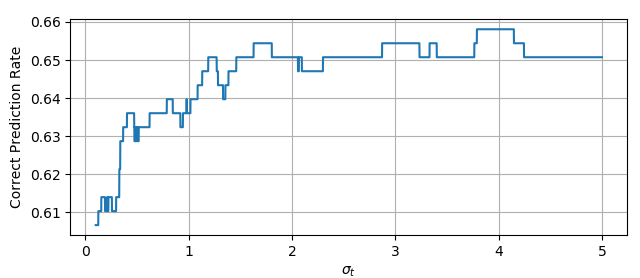
\includegraphics[width=0.7\linewidth]{grid_st_fin}
		\caption{Grid search results of finding a $ \sigma_t $ to get a higher prediction rate.}
		\label{fig:grid_search}
	\end{figure}

	An approach to allow ``draw'' as a prediction was implemented by using assigning ``draw'' if the difference $ (\mu_1-3\sigma_1) - (\mu_2 - 3\sigma_2)$ is within the range $ (-\tau, \tau) $. After some trial-and-error process of finding good $\tau$ values, a grid search was made over the range $ [0.01, 5] $ with 2000 linearly spaced values. The plot of $r$ with conservative skill estimate is shown in figure \ref{fig:grid_tau}. Although $r$ is higher than without predicting draws, it is still lower than 50\% which would be guessing at random.
	\begin{figure}[h]
		\centering
		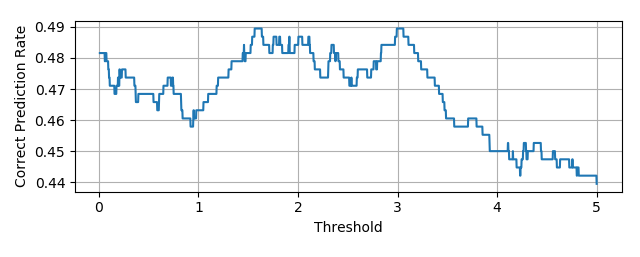
\includegraphics[width=0.7\linewidth]{grid_tau}
		\caption{Grid search of threshold values $\tau$ to find a high correct prediction rate.}
		\label{fig:grid_tau}
	\end{figure}

	This section concludes the report and leaves the problem of predicting even matches unresolved. The simplistic approaches proposed in this report did not show to be very promising for that purpose, suggesting more sophisticated or complex approaches is the way to go. 
	%%%%%%%%%%%%%%%%%%%%%%%%%%%%%%%%%%%%%%%%%%%%%%%%%%%%%%%%%%%%%%%%%%%%%%%%%%%%%%%%%%%%%%%%%%%%%%%%%%%%%%%%%%%%%%%%%%%%%%%%%%%%%%%
	\section*{Appendix}

	\subsection{Reverse Chronological Order of the SerieA Dataset}\label{app:reverse_gibbs}
	Processing the \texttt{SerieA} dataset in reverse chronological order, using Gibbs sampling results in different results than if processing was done chronologically. The reversed order results are presented in table \ref{tab:q4_rev}.
	
	\begin{table}[!h]
		\caption{Mean, variance and conservative estimate of each team's skill after all matches simulated in reverse order.}
		\label{tab:q4_rev}
		\centering
		\footnotesize
		\begin{tabular}{lrrr}
			\toprule
			\multicolumn{4}{c}{Reversed chronological order} \\
			\midrule
			Team     		& $ \mu $ & $ \sigma $ & $ \mu - 3\sigma $\\
			\midrule
			Juventus    &  33.00  &  2.05  &  26.84\\
			Napoli      &  31.31  &  2.04  &  25.17\\
			Roma        &  29.23  &  1.97  &  23.32\\
			Inter       &  28.37  &  2.25  &  21.61\\
			Torino      &  29.84  &  2.78  &  21.51\\
			Milan       &  28.12  &  2.49  &  20.65\\
			Lazio       &  26.75  &  2.23  &  20.07\\
			Sampdoria   &  25.13  &  1.75  &  19.89\\
			Atalanta    &  25.85  &  2.44  &  18.54\\
			Bologna     &  22.78  &  2.25  &  16.02\\
			Udinese     &  22.11  &  2.07  &  15.88\\
			Sassuolo    &  22.39  &  2.29  &  15.52\\
			Spal        &  21.34  &  2.36  &  14.27\\
			Parma       &  21.01  &  2.35  &  13.97\\
			Empoli      &  20.29  &  2.16  &  13.81\\
			Cagliari    &  20.24  &  2.20  &  13.64\\
			Fiorentina  &  21.07  &  2.77  &  12.75\\
			Genoa       &  20.44  &  2.74  &  12.24\\
			Frosinone   &  17.23  &  2.09  &  10.96\\
			Chievo      &  12.86  &  2.98  &   3.92\\\bottomrule
		\end{tabular}
	\end{table}
	
	\subsection{Derivation of the Message Passing Protocol for the Factor Graph in Figure \ref{fig:factor_graph}}
	\label{app:message_passing}
	The message passing is done together with moment matching for the truncated normal distribution that appears when sending the first message from factor $ f_{ty} $ to node $ t $. Other key steps are multiplications and divisions with normal distribution functions, as described in [2].
	\begin{subequations}
		\begin{align}
		&\mu_{y\rightarrow f_{ty}}(y)=\delta(y-y_\text{obs})\\
		\begin{split}
		&\mu_{f_{ty}\rightarrow t}(t) = \sum_y f_{ty}(t,y)\delta(y-y_{\text{obs}})=\\
		&=\bm{1}_{t>0,y_\text{obs}=1}+\bm{1}_{t<0,y_\text{obs}=-1}\\
		\end{split}\\
		\begin{split}
		&\text{Moment matching for the truncated Gaussian: }p(t|y)\\
		&p(t|y) \propto \mu_{f_{ty}\rightarrow t}(t)\mu_{f_{tw}\rightarrow t}(t),\\
		&\text{where}~\mu_{f_{tw}\rightarrow t}(t)\text{ computes from:}
		\end{split}\\
		\begin{split}
		&\mu_{w\rightarrow f_{tw}}(w)=\mu_{f_{sw}\rightarrow w}(w)= \\
		&\int_{s_1, s_2}f_{sw}(s_1,s_2,w)f_{s_1}(s_1)f_{s_2}(s_2)ds_1ds_2
		\end{split}\\
		&\mu_{f_{tw}\rightarrow t}(t) = \int_w f_{tw}(t,w)\mu_{f_{sw}\rightarrow w}(w)dw\\
		&\Rightarrow \hat{p}(t|y) = \mathcal{N}(t;\hat{\mu}_t, \hat{\sigma}_t^2)\\
		\begin{split}
		&\hat{\mu}_{t\rightarrow f_{tw}}(t)=\hat{\mu}_{f_{ty}\rightarrow t}(t)\\
		&= \hat{p}(t|y)/\mu_{f_{tw}\rightarrow t}(t)=\mathcal{N}(t; \hat{\mu}_{tw}, \hat{\sigma}_{tw}^2)
		\end{split}\\
		& \hat{\mu}_{f_{tw}\rightarrow w}(w) = \int_t f_{tw}(t,w)\hat{\mu}_{t\rightarrow f_{tw}}(t)dt=\mathcal{N}(w; \hat{\mu}_{w}, \hat{\sigma}_{w}^2)\\
		& \hat{\mu}_{w\rightarrow f_{sw}}(w) = \hat{\mu}_{f_{tw}\rightarrow w}(w)\\
		& \hat{\mu}_{f_{sw}\rightarrow s_1}(s_1) = \int_{w, s_2}f_{sw}(s_1,s_2,w)\hat{\mu}_{w\rightarrow f_{sw}}(w)\mu_{s_2\rightarrow f_{sw}}(s_2)\,dw\,ds_2 \label{message:sw_s1}\\
		& \hat{\mu}_{f_{sw}\rightarrow s_2}(s_2) = \int_{w, s_1}f_{sw}(s_1,s_2,w)\hat{\mu}_{w\rightarrow f_{sw}}(w)\mu_{s_1\rightarrow f_{sw}}(s_1)\,dw\,ds_1 \label{message:sw_s2}\\
		&p(s_1|y) \propto \mu_{f_{s_1}\rightarrow s_1}(s_1)\mu_{f_{sw}\rightarrow s_1}(s_1)\\
		&p(s_2|y) \propto \mu_{f_{s_2}\rightarrow s_2}(s_2)\mu_{f_{sw}\rightarrow s_2}(s_2)
		\end{align}
	\end{subequations}
	The integrals in equations \eqref{message:sw_s1} and \eqref{message:sw_s2} are computed by acknowledging that the factor $ f_{sw}(s_1,s_2,w) $ is a Dirac impulse function, so the integral over $ s_1 $ and $ s_2 $ respectively, becomes a sampling of the messages $ \mu_{s_2\rightarrow f_{sw}}(s_2=s_1-w) $ and $ \mu_{s_1\rightarrow f_{sw}}(s_1=s_2+w) $ respectively.
	The mean value $\hat{\mu}_w$ is equal to the value computed in the moment matching: $ \hat{\mu}_w = \hat{\mu}_{tw} $.
	The variance $ \hat{\sigma}_w^2 $ is equal to the sum of the variance from the moment matching and the variance of the variable $ t $: $ \hat{\sigma}_w^2=\hat{\sigma}_{tw}^2+\sigma_t^2 $.



	\section*{References}

	\small
	[1] Risuelo, R.S. (2019) ``Advanced Probabilistic Machine Learning, Lecture 3 – Bayesian Graphical Models''. Available through \url{http://www.it.uu.se/edu/course/homepage/apml/lectures/Lecture3_handout.pdf}, accessed 2019-10-03.
	
	[2] Risuelo, R.S. (2019) ``Advanced Probabilistic Machine Learning, Lecture 5 – Undirected Graphical Models''. Available through \url{http://www.it.uu.se/edu/course/homepage/apml/lectures/lecture5_handout.pdf}, accessed 2019-10-03.
	
	[3] Minka, T.\ \& Zaykov, Y.\ \& Tseran, H.\ (2005)  ``TrueSkill Ranking System''. Available through \url{https://www.microsoft.com/en-us/research/project/trueskill-ranking-system/}, accessed 2019-10-03.
	
	[4] Weisstein, E. W.\ (2019) ``Normal Distribution''. From MathWorld--A Wolfram Web Resource. \url{http://mathworld.wolfram.com/NormalDistribution.html}, accessed on 2019-10-03.
	
\end{document}

